%%%%%%%%%%%%%%%%%%%%%%%%%%%%%%%%%%%%%%%%%
% Jacobs Landscape Poster
% LaTeX Template
% Version 1.0 (29/03/13)
%
% Created by:
% Computational Physics and Biophysics Group, Jacobs University
% https://teamwork.jacobs-university.de:8443/confluence/display/CoPandBiG/LaTeX+Poster
% 
% Further modified by:
% Nathaniel Johnston (nathaniel@njohnston.ca)
%
% This template has been downloaded from:
% http://www.LaTeXTemplates.com
%
% License:
% CC BY-NC-SA 3.0 (http://creativecommons.org/licenses/by-nc-sa/3.0/)
%
%%%%%%%%%%%%%%%%%%%%%%%%%%%%%%%%%%%%%%%%%

%----------------------------------------------------------------------------------------
%	PACKAGES AND OTHER DOCUMENT CONFIGURATIONS
%----------------------------------------------------------------------------------------

\documentclass[final]{beamer}

\usepackage[scale=1.24]{beamerposter} % Use the beamerposter package for laying out the poster

\usetheme{confposter} % Use the confposter theme supplied with this template

\setbeamercolor{block title}{fg=ngreen,bg=white} % Colors of the block titles
\setbeamercolor{block body}{fg=black,bg=white} % Colors of the body of blocks
%% \setbeamercolor{block alerted title}{fg=white,bg=dblue!70} % Colors of the highlighted block titles
%% \setbeamercolor{block alerted body}{fg=black,bg=dblue!10} % Colors of the body of highlighted blocks
\setbeamercolor{block alerted title}{fg=white,bg=BlueViolet!70} % Colors of the highlighted block titles
\setbeamercolor{block alerted body}{fg=black,bg=BlueViolet!10} % Colors of the body of highlighted blocks
% Many more colors are available for use in beamerthemeconfposter.sty

%-----------------------------------------------------------
% Define the column widths and overall poster size
% To set effective sepwid, onecolwid and twocolwid values, first choose how many columns you want and how much separation you want between columns
% In this template, the separation width chosen is 0.024 of the paper width and a 4-column layout
% onecolwid should therefore be (1-(# of columns+1)*sepwid)/# of columns e.g. (1-(4+1)*0.024)/4 = 0.22
% Set twocolwid to be (2*onecolwid)+sepwid = 0.464
% Set threecolwid to be (3*onecolwid)+2*sepwid = 0.708

\newlength{\sepwid}
\newlength{\onecolwid}
\newlength{\twocolwid}
\newlength{\threecolwid}
\setlength{\paperwidth}{48in} % A0 width: 46.8in
\setlength{\paperheight}{36in} % A0 height: 33.1in
\setlength{\sepwid}{0.024\paperwidth} % Separation width (white space) between columns
\setlength{\onecolwid}{0.22\paperwidth} % Width of one column
\setlength{\twocolwid}{0.464\paperwidth} % Width of two columns
\setlength{\threecolwid}{0.708\paperwidth} % Width of three columns
\setlength{\topmargin}{-0.5in} % Reduce the top margin size
%-----------------------------------------------------------

\usepackage{graphbox}  % Required for including images

\usepackage{booktabs} % Top and bottom rules for tables

% Custom commands
\newcommand{\isot}[2]{$^{#2}\mathrm{#1}$}
\newcommand{\isotm}[2]{{}^{#2}\mathrm{#1}}

%----------------------------------------------------------------------------------------
%	TITLE SECTION 
%----------------------------------------------------------------------------------------

\title{pynucastro: Code Generation and Visualization for Nuclear Reaction Networks} % Poster title

\author{Donald E. Willcox (LBNL), Adam Jacobs (MSU), Xinlong Li (SBU), and Michael Zingale (SBU)}

\institute{Lawrence Berkeley National Laboratory (LBNL), Michigan State University (MSU), Stony Brook University (SBU)} % Institution(s)

%----------------------------------------------------------------------------------------

\begin{document}

\addtobeamertemplate{block end}{}{\vspace*{2ex}} % White space under blocks
\addtobeamertemplate{block alerted end}{}{\vspace*{2ex}} % White space under highlighted (alert) blocks

\setlength{\belowcaptionskip}{2ex} % White space under figures
\setlength\belowdisplayshortskip{2ex} % White space under equations

\begin{frame}[t] % The whole poster is enclosed in one beamer frame

\begin{columns}[t] % The whole poster consists of three major columns, the second of which is split into two columns twice - the [t] option aligns each column's content to the top

\begin{column}{\sepwid}\end{column} % Empty spacer column

\begin{column}{\onecolwid} % The first column

\begin{alertblock}{Abstract}

  pynucastro is developed to meet both pedagogical and research needs
  in the field of nuclear astrophysics by providing a Python interface
  to nuclear reaction rate databases (including the JINA Reaclib
  nuclear reaction rate database). It is meant for both interactive
  exploration of reaction rates (through Jupyter notebooks) and for
  creating reaction networks for use in simulation codes.

\end{alertblock}

%----------------------------------------------------------------------------------------
%	Capabilities
%----------------------------------------------------------------------------------------
\begin{block}{Capabilities}

\begin{itemize}
\item Supports Reaclib library snapshots
\item Supports weak rates tabulated in $\mathrm{(T, \rho Y_e)}$
\item Visualizes connections between nuclei as a network graph
\item Evaluates rates as a function of temperature
\item Symbolically constructs the ODE right hand side and Jacobian
\item Generates Python or Fortran code implementing the network
\end{itemize}

\end{block}

%----------------------------------------------------------------------------------------
%	Reaclib Rates
%----------------------------------------------------------------------------------------

\begin{block}{Working with Reaclib}

pynucastro can interpret reaction rates parameterized in the standard
Reaclib formats \cite{Reaclib.2010}, storing each rate internally
using the \textbf{Rate} class. \textbf{Rate} interprets the Reaclib
format and knows how to evaluate the rate as a function of
temperature.

\begin{figure}
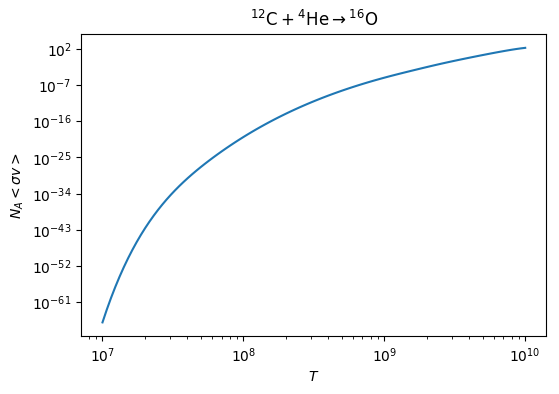
\includegraphics[width=\linewidth]{figures/library-examples-filtering_cago.png}
%\caption{Temperature dependence of $\isotm{C}{12} + \isotm{He}{4} \rightarrow \isotm{O}{16}$}
\end{figure}

\end{block}
%----------------------------------------------------------------------------------------

\end{column} % End of the first column

\begin{column}{\sepwid}\end{column} % Empty spacer column

\begin{column}{\twocolwid} % Begin a column which is two columns wide (column 2)

\begin{columns}[t,totalwidth=\twocolwid] % Split up the two columns wide column

\begin{column}{\onecolwid}\vspace{-.6in} % The first column within column 2 (column 2.1)

%----------------------------------------------------------------------------------------
%	Creating a Network
%----------------------------------------------------------------------------------------

\begin{block}{Creating a Network}

The \textbf{Library} class allows pynucastro to work easily with files
containing multiple rates, including Reaclib snapshots. We use
\textbf{Library} to obtain the CNO rates linking our desired nuclei in
just a few lines of Python in the following Jupyter notebook:

\begin{figure}
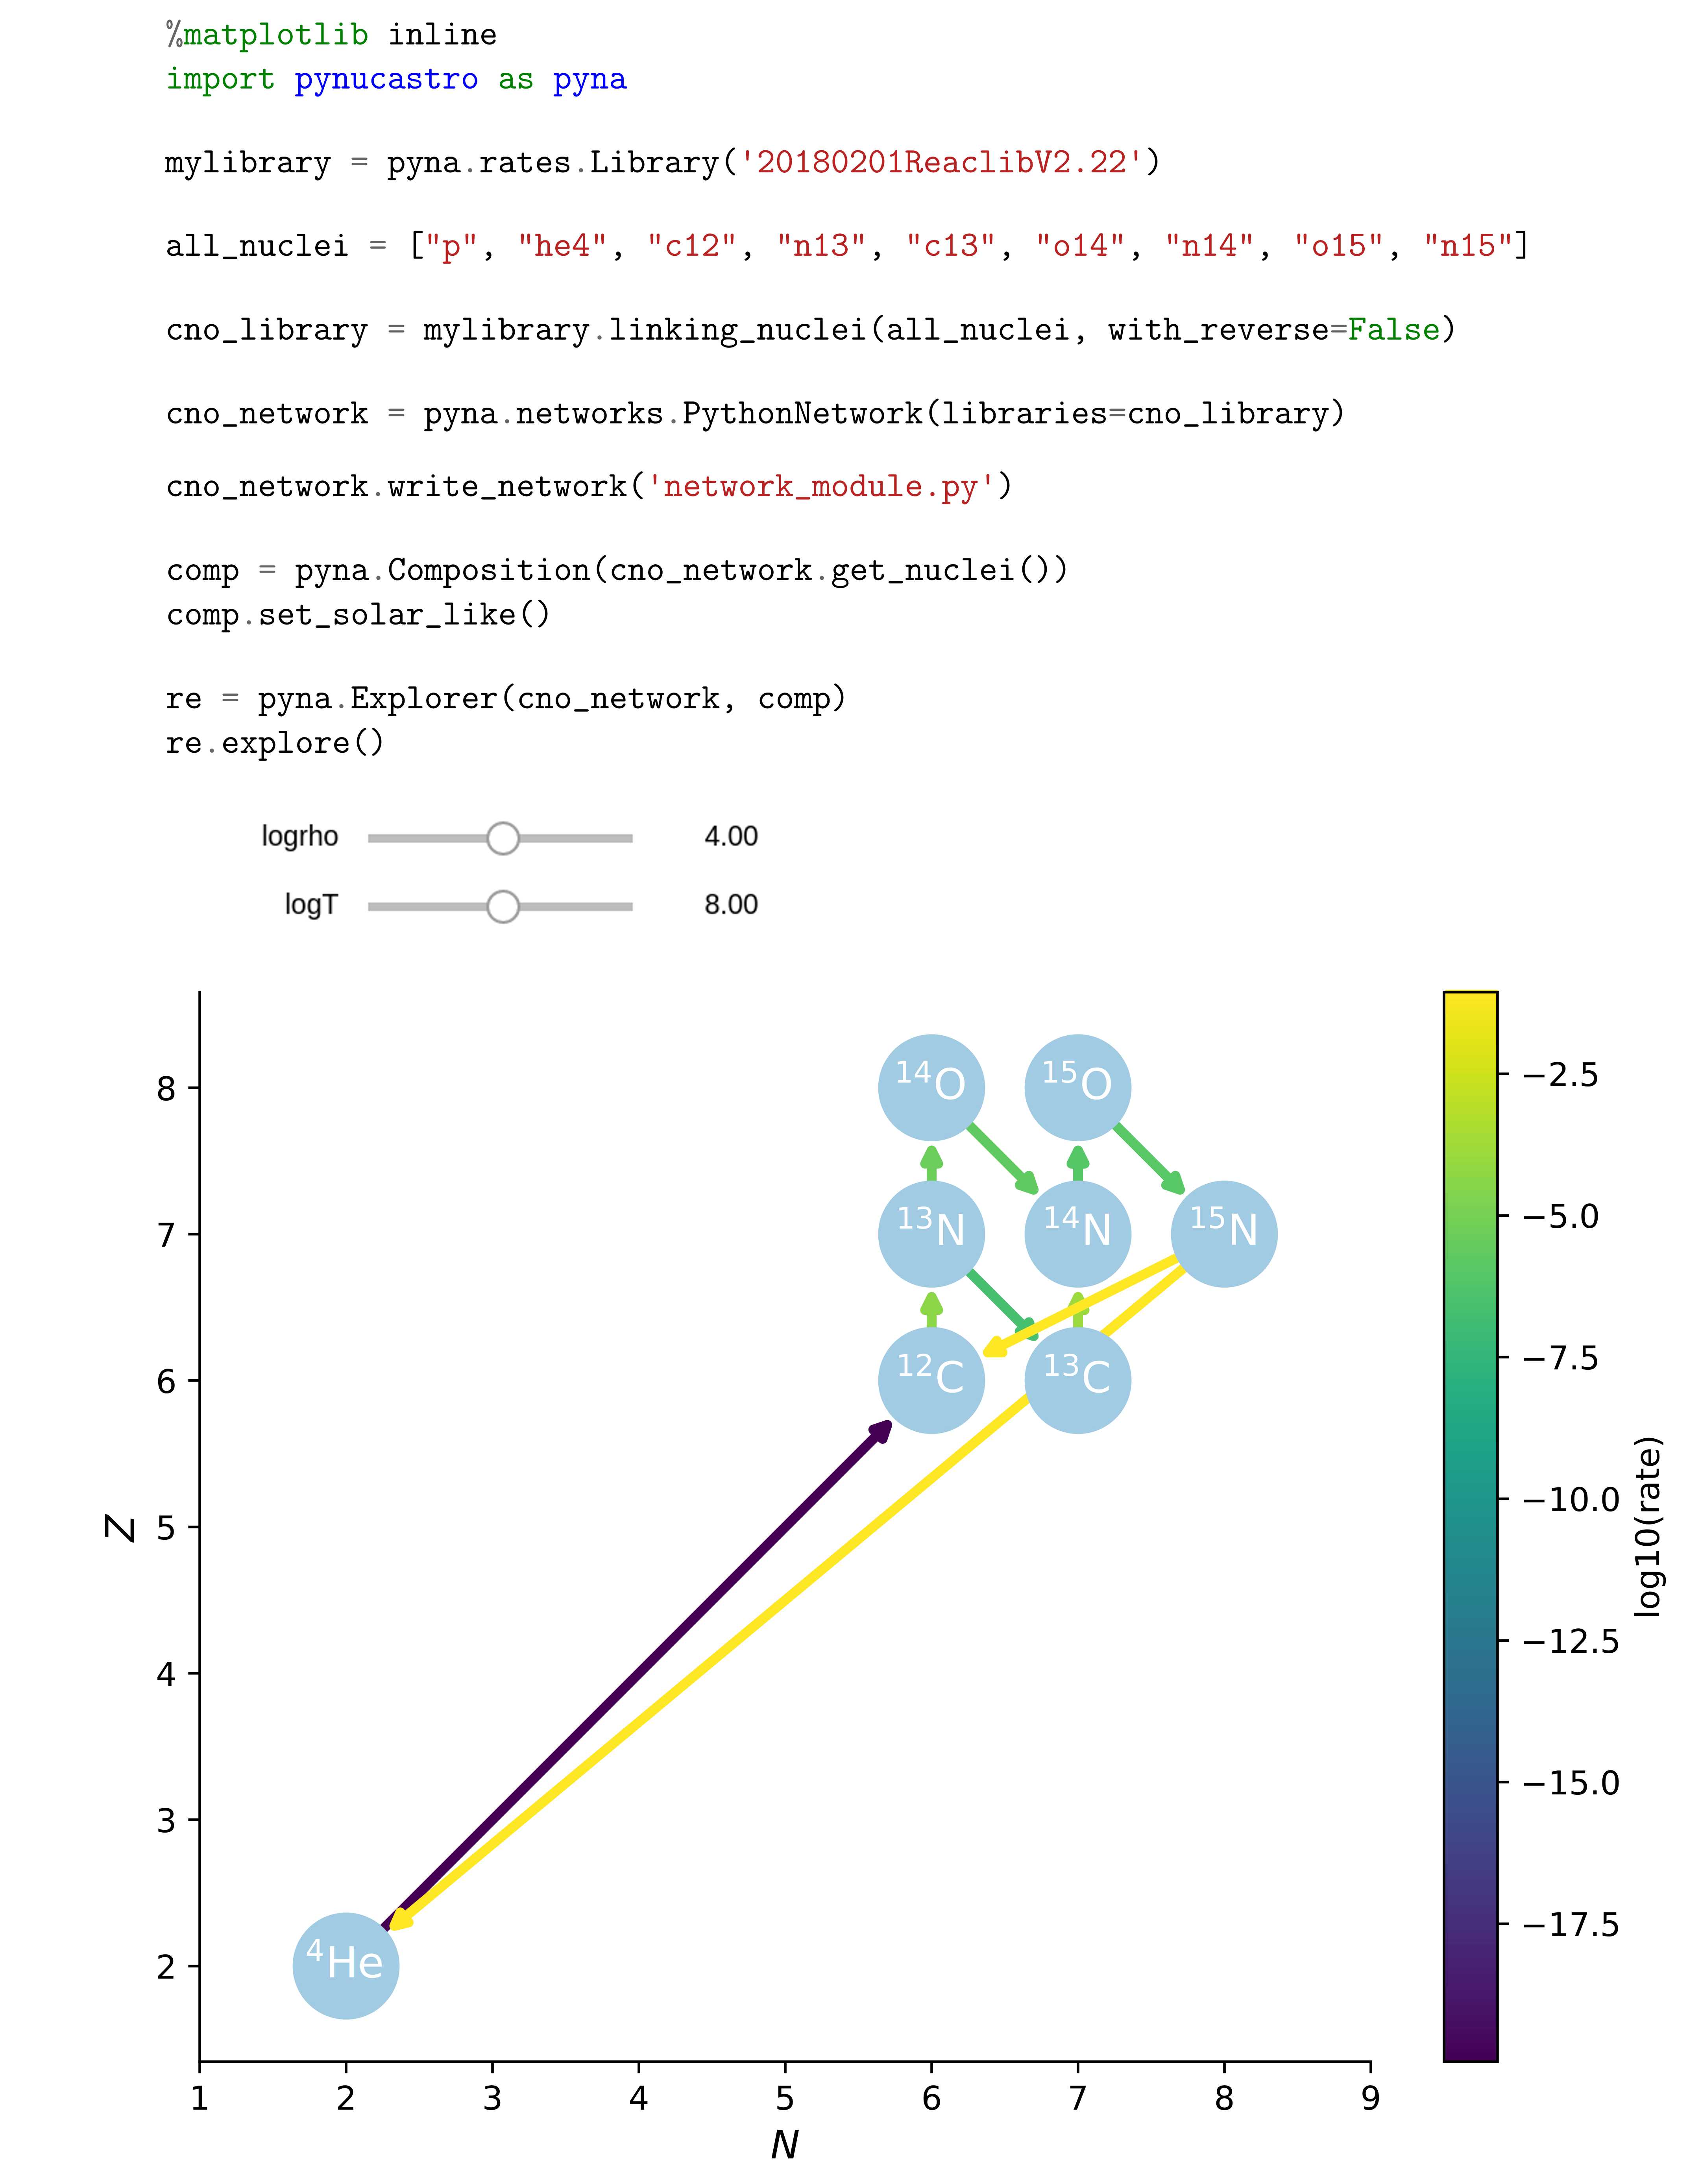
\includegraphics[width=1.1\linewidth]{figures/library-examples-nuclei.png}
%\caption{Creating a CNO network in a Jupyter notebook}
\end{figure}

Using the \textbf{Composition} and \textbf{Explorer} classes, we also
construct an interactive graph of the network with the value of each
rate indicated by its arrow color with variable density and temperature.

\end{block}

\begin{block}{Python Code Generation}

The \textbf{PythonNetwork} class generates Python code to calculate
each rate as a function of temperature and the ODE right hand
side. pynucastro includes a sample Python integrator using SciPy.

%% \begin{figure}
%% 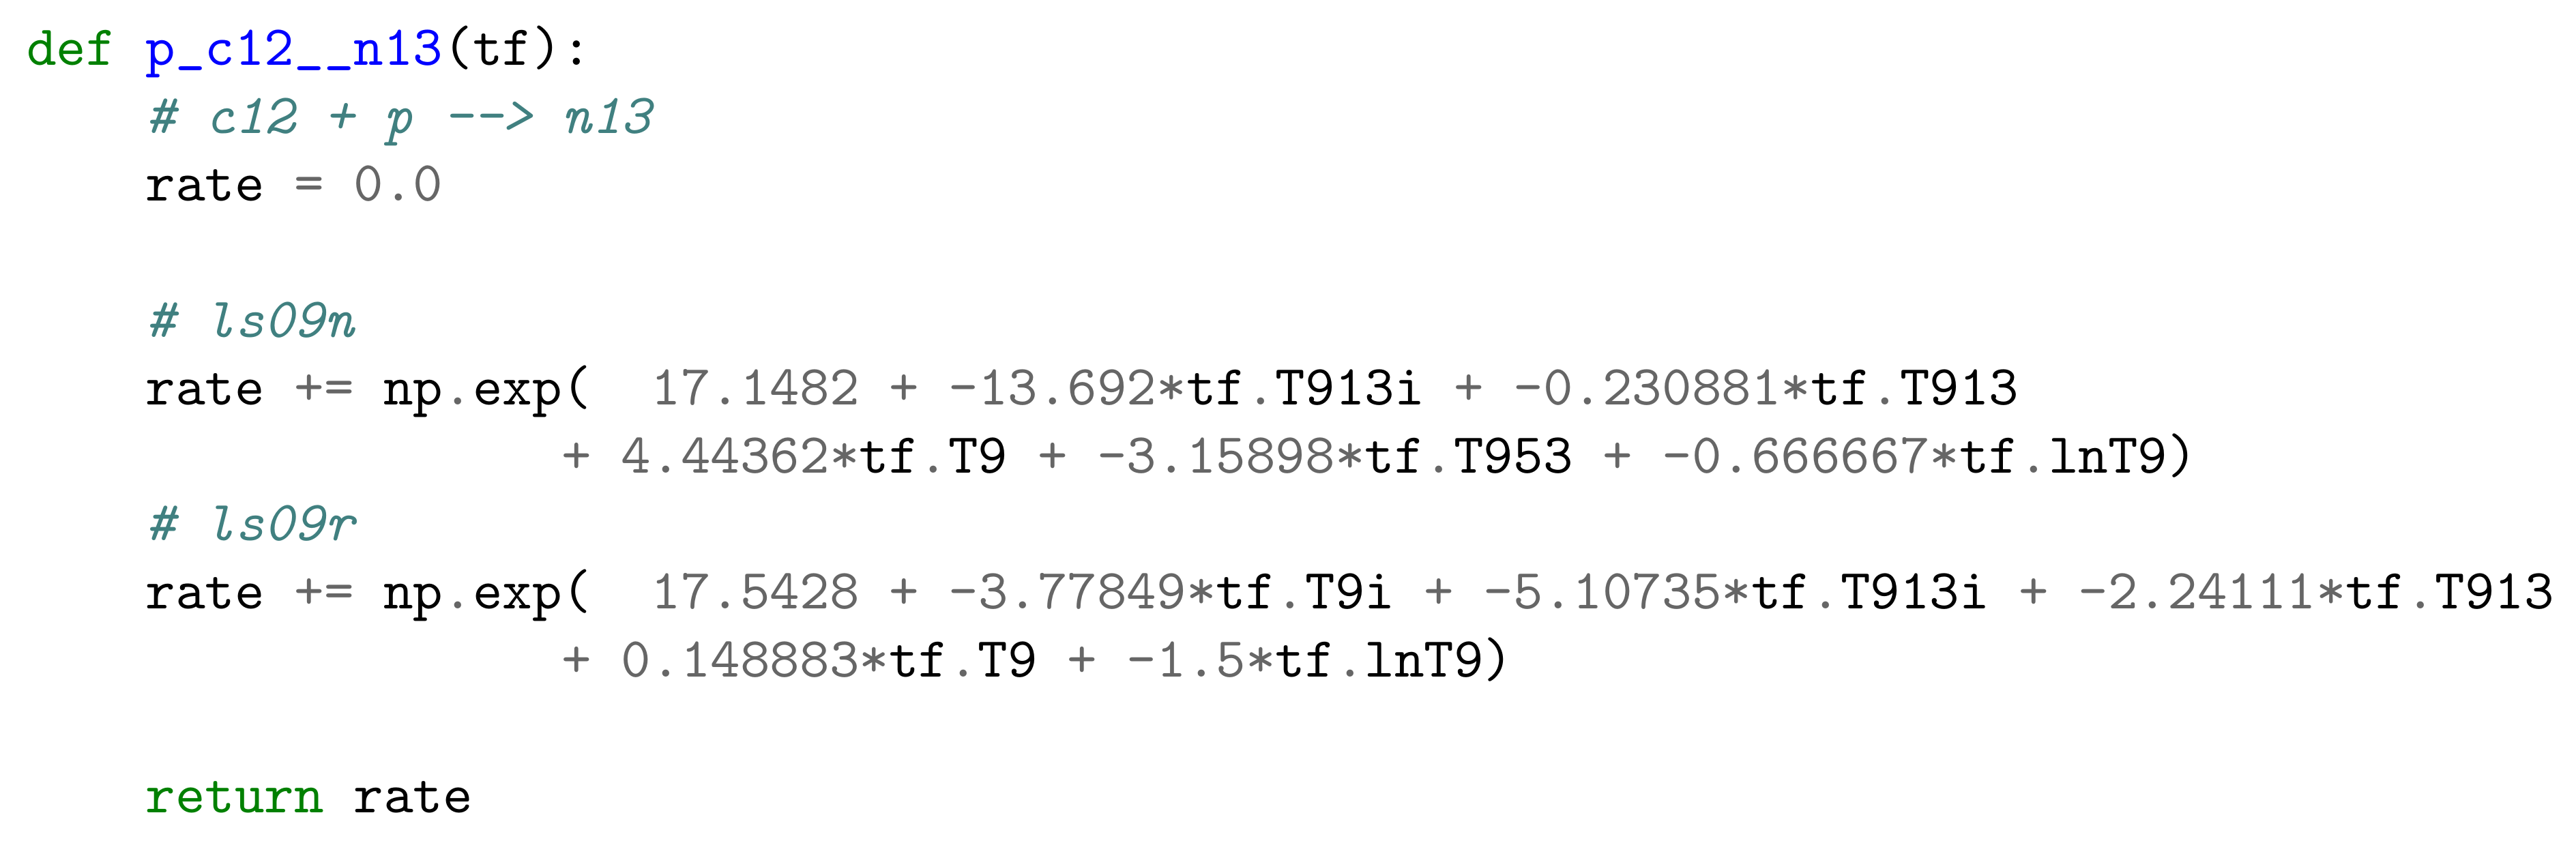
\includegraphics[width=0.8\linewidth]{figures/python-network-code/python-network-code.png}
%% %\caption{Python code evaluating the Reaclib rate for  $\isotm{C}{12} + p \rightarrow \isotm{N}{13}$}
%% \end{figure}

\end{block}

%----------------------------------------------------------------------------------------

\end{column} % End of column 2.1

\begin{column}{\onecolwid}\vspace{-.6in} % The second column within column 2 (column 2.2)

%----------------------------------------------------------------------------------------
%	Code Generation
%----------------------------------------------------------------------------------------

%% pynucastro provides several classes for generating code to calculate
%% the right hand side of the system of differential equations comprising
%% the reaction network.


\begin{block}{Fortran Code Generation}

The \textbf{BaseFortranNetwork} class uses 

\begin{figure}
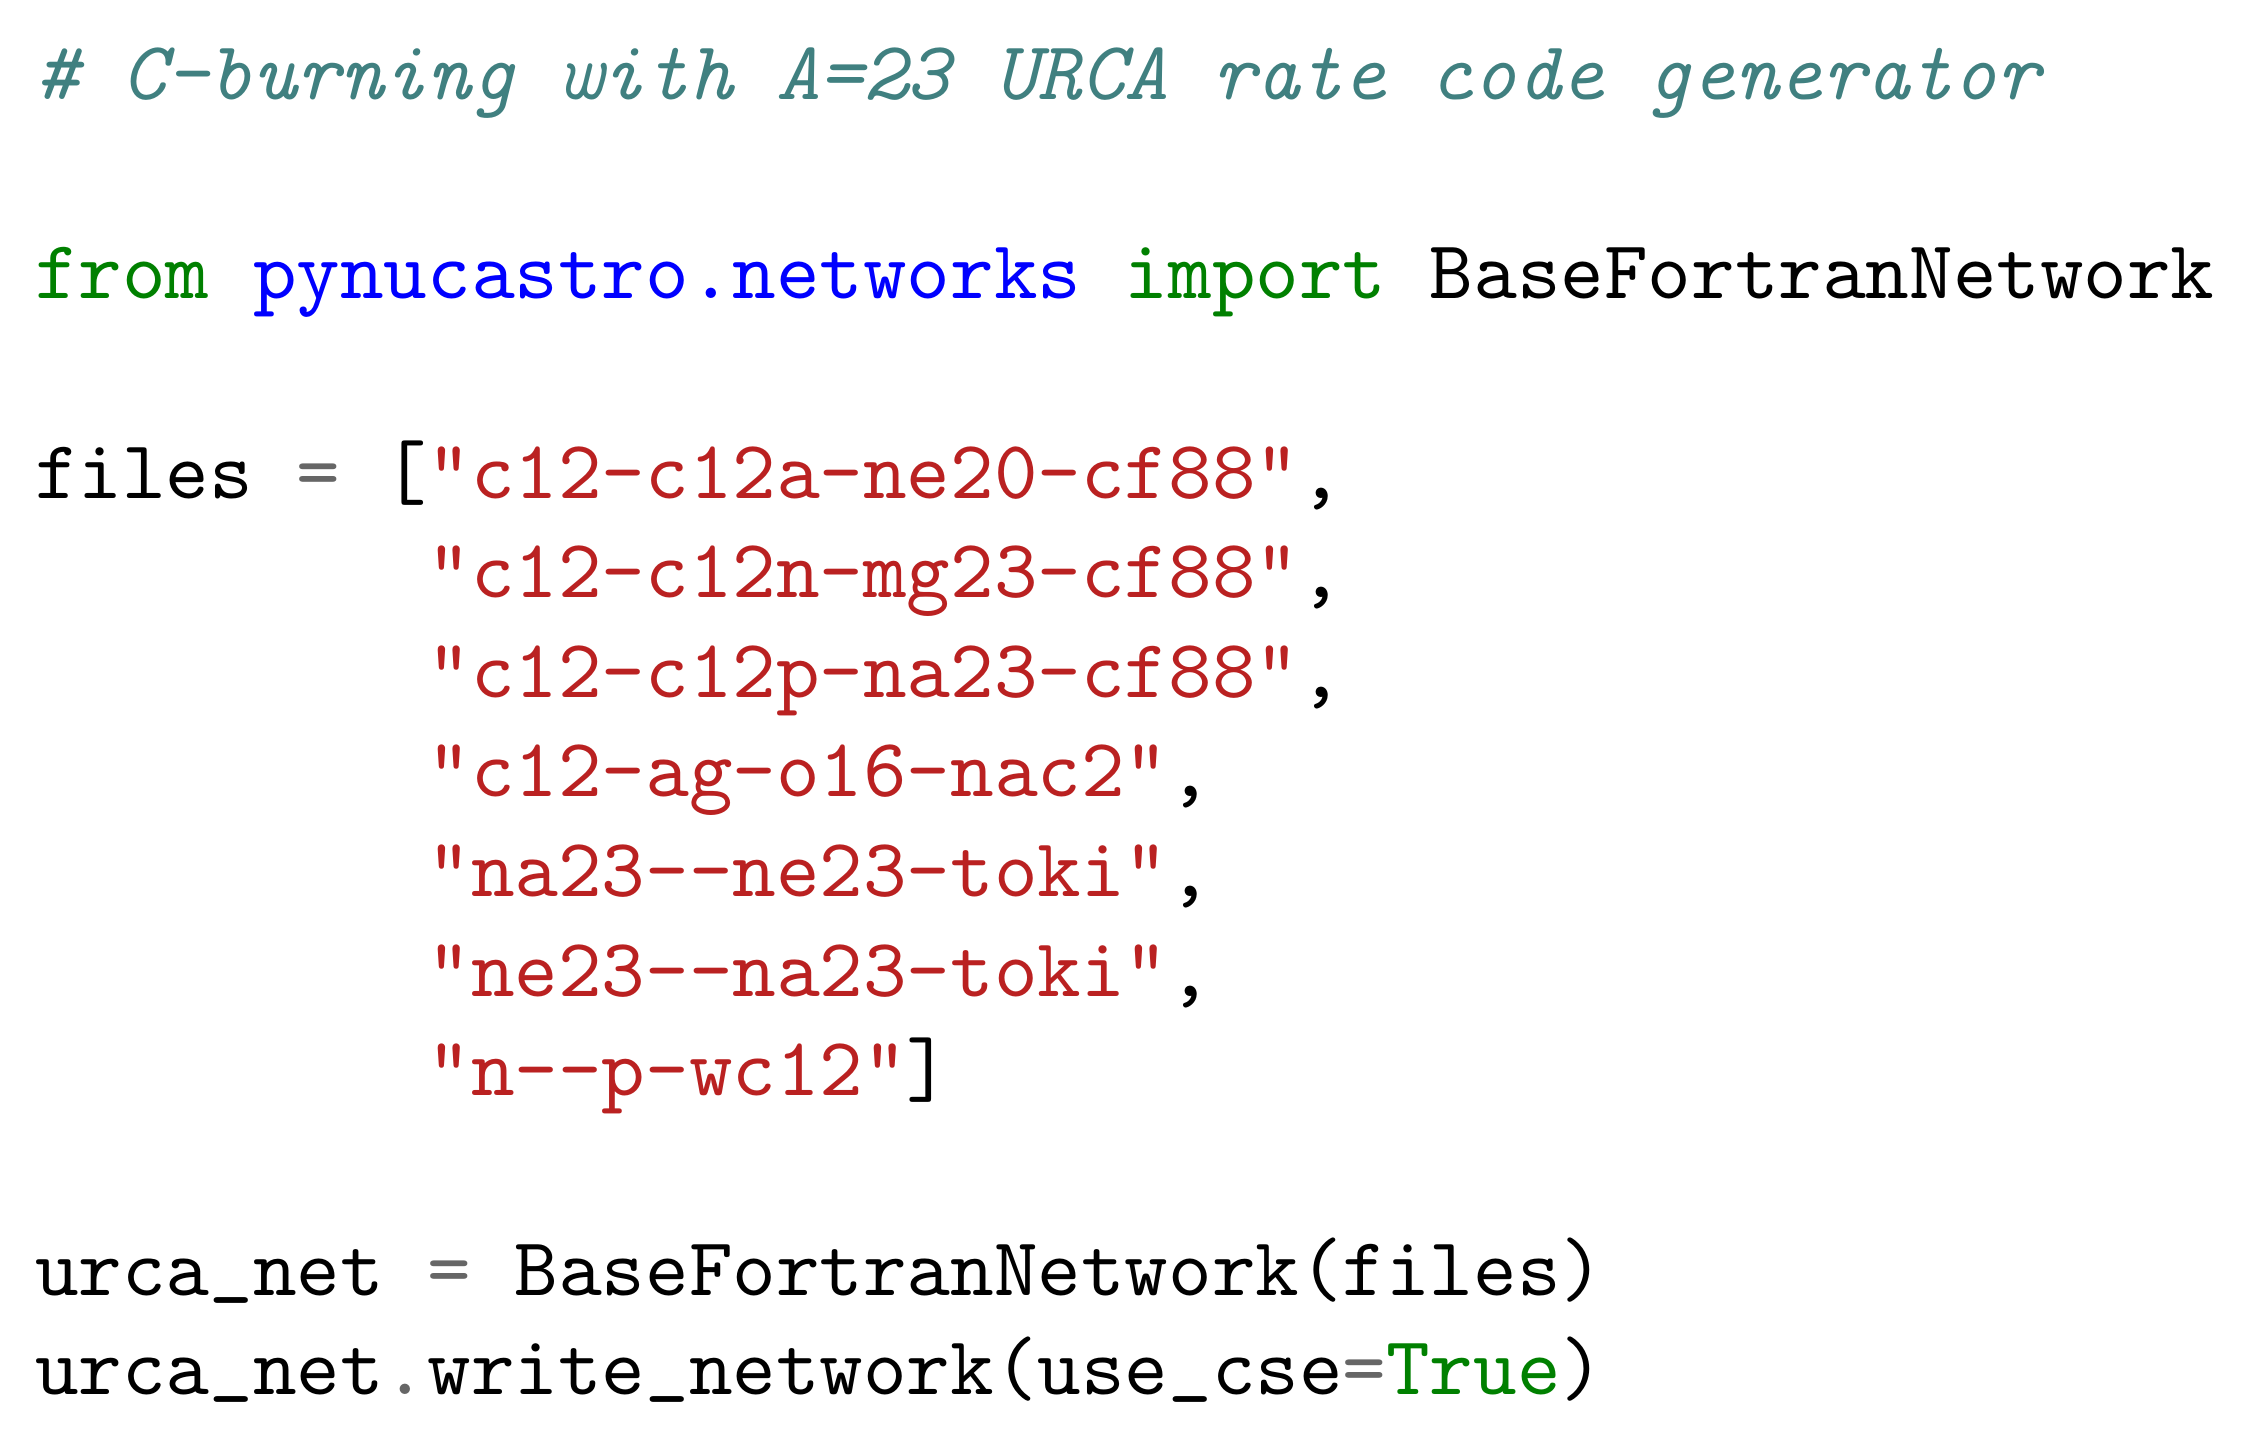
\includegraphics[width=0.8\linewidth]{figures/basefortran-network/basefortrannetwork.png}
%\caption{Constructing a Fortran implementation of an $\mathrm{A=23}$ Urca network with \isot{C}{12} burning.}
\end{figure}

\end{block}


\begin{block}{StarKiller Microphysics}

The \textbf{StarKillerNetwork} class generates Fortran reaction
network code for astrophysical simulations that use the StarKiller
Microphysics repository \cite{Zingale.astronum.2017}.

\begin{itemize}
    \item Uses Sympy \cite{SymPy.2017}
    \item Derives right hand side and Jacobian matrix
    \item Couples to physics modules in StarKiller
    \begin{itemize}
        \item stellar EOS
        \item reaction screening
        \item thermal neutrino rates
    \end{itemize}
    \item Supports CUDA Fortran
\end{itemize}

Electron fraction in a MAESTRO low-Mach hydrodynamics simulation of a
convecting white dwarf core using the $\mathrm{A=23}$ Urca network:

\begin{figure}
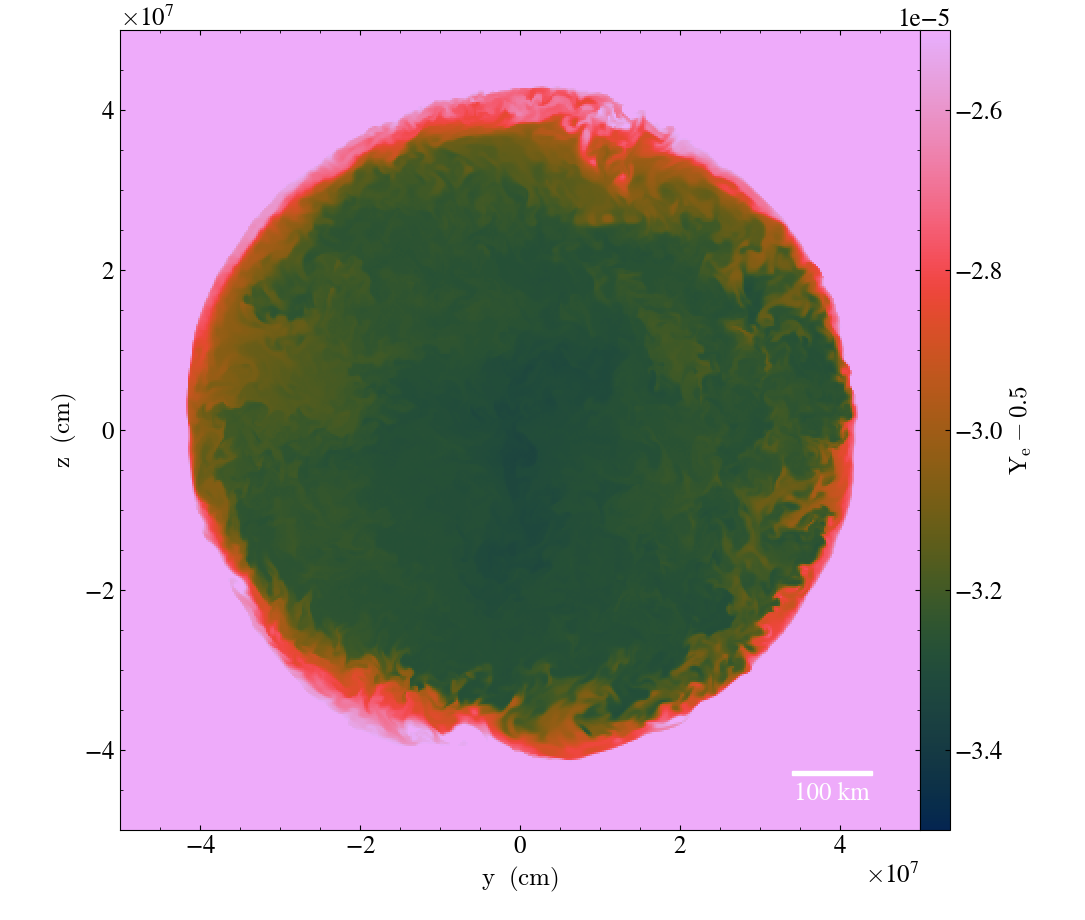
\includegraphics[width=\linewidth]{figures/starkiller-network/wd_4lev_Tc5-5e8_rhoc4-5e9_plt06605_slice_x_electron_fraction_asymmetry.png}
%\caption{Electron fraction in a MAESTRO low-Mach hydrodynamics simulation of a convecting white dwarf core using the $\mathrm{A=23}$ Urca network with \isot{C}{12} burning.}
\end{figure}

\end{block}

%----------------------------------------------------------------------------------------

\end{column} % End of column 2.2

\end{columns} % End of the split of column 2 - any content after this will now take up 2 columns width

% %----------------------------------------------------------------------------------------
% %	IMPORTANT RESULT
% %----------------------------------------------------------------------------------------

% \begin{alertblock}{Important Result}

% Lorem ipsum dolor \textbf{sit amet}, consectetur adipiscing elit. Sed commodo molestie porta. Sed ultrices scelerisque sapien ac commodo. Donec ut volutpat elit.

% \end{alertblock} 

%----------------------------------------------------------------------------------------

\end{column} % End of the second column

\begin{column}{\sepwid}\end{column} % Empty spacer column

\begin{column}{\onecolwid} % The third column

%----------------------------------------------------------------------------------------
%	Getting pynucastro
%----------------------------------------------------------------------------------------

\setbeamercolor{block title}{fg=BlueViolet,bg=white} % Change the block title color
  
\begin{block}{Getting pynucastro}

\begin{itemize}
\item pynucastro is freely available under the \textbf{BSD 3-Clause open source} license.
\item For the companion \textbf{software paper}, see \cite{pynucastro.joss.2018}.
\item Visit us on GitHub to \textbf{download} pynucastro or report \textbf{issues} and request features:
\end{itemize}

\url{https://github.com/pynucastro/pynucastro}

\begin{itemize}
\item For pynucastro \textbf{documentation} and examples, visit the pynucastro website:
\end{itemize}

\url{https://pynucastro.github.io/pynucastro}

\end{block}

%----------------------------------------------------------------------------------------
%	ACKNOWLEDGEMENTS
%----------------------------------------------------------------------------------------

\setbeamercolor{block title}{fg=ngreen,bg=white} % Colors of the block titles

\begin{block}{Acknowledgements}

\small{\rmfamily{This work was supported by DOE/Office of Nuclear
    Physics grant DE-FG02-87ER40317. This research used resources of
    the Oak Ridge Leadership Computing Facility, which is a DOE Office
    of Science User Facility supported under Contract
    DE-AC05-00OR22725.}}

\end{block}

%----------------------------------------------------------------------------------------
%	REFERENCES
%----------------------------------------------------------------------------------------

\begin{block}{References}

%\nocite{*} % Insert publications even if they are not cited in the poster
\small{\bibliographystyle{customunsrt}
\bibliography{paper}\vspace{0.75in}}

\end{block}

%% %----------------------------------------------------------------------------------------
%% %	CONTACT INFORMATION
%% %----------------------------------------------------------------------------------------

%% \setbeamercolor{block alerted title}{fg=black,bg=norange} % Change the alert block title colors
%% \setbeamercolor{block alerted body}{fg=black,bg=white} % Change the alert block body colors

%% \begin{alertblock}{Contact Information}

%% \begin{itemize}
%% \item Web: \href{https://dwillcox.github.io}{https://dwillcox.github.io}
%% \item Email: \href{mailto:donald.willcox@stonybrook.edu}{donald.willcox@stonybrook.edu}
%% \item Phone: +1 (631) 632-8236
%% \end{itemize}

%% \end{alertblock}

%----------------------------------------------------------------------------------------

\end{column} % End of the third column

\end{columns} % End of all the columns in the poster

\end{frame} % End of the enclosing frame

\end{document}
